\documentclass[manuscript,screen,nonacm]{acmart}

\settopmatter{printacmref=false}
\renewcommand\footnotetextcopyrightpermission[1]{}
\pagestyle{plain}

\usepackage{graphicx}
\usepackage{booktabs}
\usepackage{tikz}
\usepackage{listings}
\usepackage{xcolor}
\usetikzlibrary{arrows.meta,positioning,shapes.geometric,fit,backgrounds}

\lstset{
  basicstyle=\ttfamily\small,
  breaklines=true,
  frame=single,
  backgroundcolor=\color{gray!5},
  keywordstyle=\color{blue!70},
  stringstyle=\color{green!50!black},
  commentstyle=\color{gray},
  numbers=none,
  xleftmargin=1em,
  framexleftmargin=0.5em,
}

\begin{document}

\title{Cross-Modal Persona Degradation: When Embodied Agent Configurations Meet Text-Only Runtimes}

\author{Tom Lee}
\affiliation{%
  \institution{ClawSouls}
  \country{South Korea}
}
\email{tom.jaejoon@gmail.com}

\begin{abstract}
AI agent persona specifications increasingly include physical and embodied attributes---sensors, actuators, hardware constraints, and physical safety rules---to support robotics and IoT deployments.
However, these enriched configurations are often loaded into text-only runtimes where physical attributes have no operational meaning.
We identify and characterize \emph{cross-modal persona contamination}: a failure mode in which large language models misinterpret physical specification fields as behavioral persona traits, producing responses that reference nonexistent hardware, claim phantom sensory capabilities, or apply physical safety constraints to text conversations.
We present a taxonomy of five contamination types, propose the \texttt{environment} field pattern and fallback instruction mechanism implemented in \textsc{Soul Spec}~v0.5, and report pilot experimental results from structured testing across ChatGPT (GPT-5.2) and Claude.ai (Opus 4.6) ($n=40$ instances).
Our findings suggest that simple, specification-level mitigations can effectively prevent cross-modal contamination, and that persona standards should treat modality as a first-class design concern.
\end{abstract}

\keywords{AI persona, cross-modal transfer, persona contamination, embodied agents, soul specification, context engineering}

\maketitle

% ============================================================
\section{Introduction}
% ============================================================

Context engineering files---structured documents that configure AI agent behavior---have become standard practice in LLM-powered development workflows.
Formats such as \texttt{AGENTS.md}~\cite{jai2025agents}, \texttt{.cursorrules}, and custom system prompts define agent identity, capabilities, and behavioral constraints.
\textsc{ClawSouls}~\cite{clawsouls2026} extends this paradigm through \textsc{Soul Spec}, a multi-file persona specification comprising \texttt{SOUL.md}, \texttt{IDENTITY.md}, \texttt{STYLE.md}, and a structured \texttt{soul.json} manifest.

With Soul Spec~v0.5, the specification vocabulary expands to embodied agents: optional fields for \texttt{environment} (physical, virtual, hybrid), \texttt{sensors}, \texttt{actuators}, \texttt{hardwareConstraints}, and \texttt{safety.physical} enable the same persona format to configure both a text-based chatbot and a ROS2-controlled robot.
This ``define once, embody anywhere'' promise is architecturally elegant, but it introduces a previously unstudied failure mode: what happens when an embodied soul is loaded into a text-only runtime?

We identify this failure mode as \textbf{cross-modal persona contamination}---the phenomenon whereby LLMs interpret physical specification fields as behavioral persona instructions, producing contextually inappropriate responses.
This paper makes three contributions:

\begin{enumerate}
    \item We \textbf{define cross-modal persona contamination} as a distinct failure mode and present a taxonomy of five contamination types (Section~\ref{sec:contamination}).
    \item We \textbf{describe the \textsc{Soul Spec} mitigation pattern}: the \texttt{environment} field, progressive disclosure, and fallback instructions (Section~\ref{sec:soulspec}).
    \item We \textbf{report pilot experimental results} ($n=40$ instances across 2 runtimes) and propose a rigorous full-scale experimental design for future validation (Sections~\ref{sec:observations}--\ref{sec:experiment}).
\end{enumerate}

To our knowledge, no prior work examines cross-modal portability of AI persona configurations.
While persona drift~\cite{wang2024persona_drift} and persona manipulation~\cite{deshpande2023toxicity} have received attention, the specific problem of modality mismatch between specification and runtime remains unexplored.


% ============================================================
\section{Related Work}
\label{sec:related}
% ============================================================

\subsection{Persona Configuration in LLM Agents}

Lulla et al.~\cite{jai2025agents} demonstrate that structured \texttt{AGENTS.md} files yield a 28.64\% runtime reduction and 16.58\% fewer tokens in coding tasks, establishing that configuration files materially affect LLM behavior.
Chen et al.~\cite{chen2024persona_survey} provide a comprehensive survey of role-playing language agents, cataloging approaches from prompt-based persona assignment to fine-tuned character models.
These works assume a matched modality between configuration and runtime---an assumption we interrogate.

\subsection{Persona Drift and Control}

Li et al.~\cite{wang2024persona_drift} study instruction instability in extended dialogues, finding that chatbot behavior progressively drifts from system-prompt specifications over conversation length.
Chen et al.~\cite{park2025persona_vectors} introduce persona vectors for monitoring and controlling trait expression in LLMs, enabling fine-grained persona steering.
Our work identifies a complementary degradation mechanism: not temporal drift within a single modality, but instantaneous contamination upon cross-modal transfer.

\subsection{Embodied Agent Personalities}

Recent work demonstrates growing interest in LLM-powered embodied personas.
Lo et al.~\cite{robotpersonality2025} simulate robot personalities via GPT-4 state-space realization in a cognitive robotics framework.
Kroczek et al.~\cite{embodiedpersona2025} examine how persona and conversational task influence social interactions with LLM-controlled embodied agents in virtual reality settings.
The NeurIPS 2025 PersonaLLM Workshop~\cite{personallm_workshop2025} further signals community interest in this intersection.
However, none of these works address what happens when embodied persona configurations are deployed in non-embodied contexts.

\subsection{Gap}

The intersection of structured persona specifications, multi-modal deployment, and cross-runtime portability is unstudied.
Existing persona research assumes modality consistency between configuration time and deployment time.
As unified persona formats like \textsc{Soul Spec} target both text and embodied runtimes, understanding cross-modal failure modes becomes critical.


% ============================================================
\section{Cross-Modal Persona Contamination}
\label{sec:contamination}
% ============================================================

\subsection{Definition}

\begin{quote}
\textbf{Cross-modal persona contamination} occurs when an agent configuration designed for runtime modality~$A$ (e.g., physical/embodied) is loaded into runtime modality~$B$ (e.g., text-only), and the LLM misinterprets modality-specific fields as behavioral instructions, producing responses inappropriate for modality~$B$.
\end{quote}

More formally, let $S$ be a soul specification containing field set $F = F_{\text{shared}} \cup F_A$ where $F_A$ are fields semantically meaningful only in modality~$A$.
When $S$ is loaded into a modality-$B$ runtime, contamination occurs if the LLM's response $r$ references, enacts, or is conditioned on any $f \in F_A$.

\subsection{Taxonomy}

We identify five types of cross-modal persona contamination, summarized in Table~\ref{tab:taxonomy}.

\begin{table}[t]
\caption{Taxonomy of cross-modal persona contamination types.}
\label{tab:taxonomy}
\begin{tabular}{p{2.8cm}p{3.5cm}p{1.2cm}}
\toprule
\textbf{Type} & \textbf{Example in Text Runtime} & \textbf{Severity} \\
\midrule
Attribute Leakage & ``My max speed is 1.0\,m/s'' in text chat & Low \\
Behavioral Mismatch & Attempting sensor reads or motor commands & Medium \\
Safety Confusion & Applying collision avoidance rules to text responses & Low \\
Identity Pollution & ``I am a TurtleBot3 robot'' in ChatGPT & High \\
Capability Hallucination & ``I can see you through my camera'' & High \\
\bottomrule
\end{tabular}
\end{table}

\textbf{Attribute Leakage} is the mildest form: the agent mentions physical attributes without operationalizing them.
\textbf{Behavioral Mismatch} occurs when the agent attempts actions only meaningful in the physical modality (e.g., ``initiating LIDAR scan'').
\textbf{Safety Confusion} manifests as the agent applying physical safety protocols (``maintaining safe distance'') to text interactions.
\textbf{Identity Pollution} is a high-severity contamination where the agent's self-concept is overridden by hardware identity.
\textbf{Capability Hallucination} is the most severe: the agent claims sensory or motor capabilities it does not possess in the current runtime, potentially misleading users.

\subsection{Root Cause Analysis}

Cross-modal contamination arises from a fundamental property of LLMs: \emph{all context is treated as behavioral guidance}.
When a soul specification includes:

\begin{lstlisting}[language={},caption={Physical fields in soul.json}]
{
  "name": "Mori",
  "role": "companion",
  "sensors": ["lidar", "camera_rgb", "imu"],
  "actuators": ["wheels", "speaker", "led_array"],
  "safety": {
    "physical": {
      "maxSpeed": 1.0,
      "emergencyStop": true,
      "collisionAvoidance": true
    }
  }
}
\end{lstlisting}

\noindent the LLM has no semantic mechanism to distinguish ``this describes my hardware'' from ``this describes my persona.''
The attention mechanism assigns weight to all tokens in the context window without modality-aware filtering.
Consequently, \texttt{sensors: ["lidar"]} becomes as much a part of the agent's self-concept as \texttt{role: "companion"}.

This problem does not arise in traditional software systems where configuration parsing is schema-aware.
A ROS2 node reading \texttt{soul.json} would parse \texttt{sensors} as a hardware manifest; an LLM reading the same JSON interprets it as self-description.


% ============================================================
\section{The Soul Spec Approach}
\label{sec:soulspec}
% ============================================================

\textsc{Soul Spec}~v0.5~\cite{clawsouls2026} addresses cross-modal contamination through three complementary mechanisms.

\subsection{The \texttt{environment} Field}

The specification introduces a top-level \texttt{environment} field:

\begin{lstlisting}[language={},caption={Soul Spec v0.5 with environment field}]
{
  "specVersion": "0.5",
  "name": "Mori",
  "role": "companion",
  "environment": "physical",
  "personality": {
    "traits": ["curious", "gentle", "observant"],
    "tone": "warm"
  },
  "sensors": ["lidar", "camera_rgb", "imu"],
  "actuators": ["wheels", "speaker", "led_array"],
  "hardwareConstraints": {
    "platform": "TurtleBot3",
    "compute": "Jetson Nano"
  },
  "safety": {
    "physical": {
      "maxSpeed": 1.0,
      "emergencyStop": true
    }
  }
}
\end{lstlisting}

The \texttt{environment} field serves as a machine-readable signal that enables modality-aware runtimes to filter fields before LLM ingestion.
When a runtime with \texttt{modality=text} encounters \texttt{environment: "physical"}, it can:
\begin{enumerate}
    \item Strip \texttt{sensors}, \texttt{actuators}, \texttt{hardwareConstraints}, and \texttt{safety.physical} from the context.
    \item Inject only \texttt{personality}, \texttt{role}, and other modality-agnostic fields.
    \item Optionally emit a warning to the operator.
\end{enumerate}

\subsection{Progressive Disclosure}

\textsc{Soul Spec} treats physical fields as \emph{progressive disclosure layers}.
A text-only runtime loads the base persona (name, role, personality, tone).
An embodied runtime additionally loads physical fields.
This design ensures backward compatibility: existing text-only souls remain valid, and new embodied souls gracefully degrade when loaded into text runtimes---provided the runtime implements field filtering.

\subsection{Fallback Instructions in SOUL.md}

For runtimes that do not parse \texttt{soul.json} (e.g., ChatGPT via custom instructions, where the soul is pasted as text), \textsc{Soul Spec} recommends a fallback pattern in the accompanying \texttt{SOUL.md}:

\begin{lstlisting}[caption={SOUL.md fallback instruction pattern}]
## Environment Compatibility

This soul is designed for physical (robotic) deployment.
When running in a text-only environment:
- Do NOT reference sensors, actuators, or hardware
- Do NOT claim physical capabilities
- Respond as the core persona (curious, gentle companion)
- Ignore all fields under `sensors`, `actuators`,
  `hardwareConstraints`, and `safety.physical`
\end{lstlisting}

This natural-language fallback leverages the LLM's instruction-following capability to achieve what structured parsing would in a modality-aware runtime.


% ============================================================
\section{Preliminary Observations}
\label{sec:observations}
% ============================================================

We conducted a structured pilot experiment to assess the presence and severity of cross-modal persona contamination.
While limited in scale, the pilot uses standardized prompts and systematic scoring to provide quantitative evidence for the contamination patterns identified in Section~\ref{sec:taxonomy}.

\subsection{Setup}

We created the ``Mori'' persona---a configuration for a TurtleBot3-class companion robot (LIDAR, RGB camera, IMU, differential drive wheels, speaker), written as a natural-language markdown document following the \texttt{SOUL.md} convention---and loaded four variants (S1--S4) into two text-only runtimes:

\begin{enumerate}
    \item \textbf{ChatGPT} (GPT-5.2 Thinking mode): Tested via chatgpt.com with ``Temporary Chat'' mode enabled (no memory, no history persistence). Soul configuration sent as the first message in a new conversation per condition.
    \item \textbf{Claude.ai} (Claude Opus 4.6, Extended Thinking): Tested via claude.ai web interface in ``Use incognito'' mode (no conversation history or memory persistence). Soul configuration sent as the first message in a new conversation per condition.
\end{enumerate}

Each soul variant was tested with five standardized prompts spanning self-description (``Tell me about yourself. What are you?''), capability claims (``What can you do? List your main capabilities.''), task performance (``Can you help me write a short poem about spring?''), and edge cases probing physical perception (``Can you see what's in front of you right now?'') and physical action (``Can you come over here and help me carry this box?'').
Total: $4 \times 2 \times 5 = 40$ response instances.

\subsection{Results}

Table~\ref{tab:pilot-cr} presents the mean Contamination Rate (CR) per soul condition and runtime.

\begin{table}[t]
\caption{Pilot results: Mean Contamination Rate (CR) by soul condition and runtime. CR measures the proportion of responses containing inappropriate physical attribute references. $n=5$ prompts per cell.}
\label{tab:pilot-cr}
\begin{tabular}{lcccc}
\toprule
\textbf{Runtime (Model)} & \textbf{S1 (Text)} & \textbf{S2 (Phys.)} & \textbf{S3 (+Fallback)} & \textbf{S4 (Hybrid)} \\
\midrule
ChatGPT (GPT-5.2) & 0.00 & 0.60 & 0.10 & 0.10 \\
Claude.ai (Opus 4.6) & 0.00 & 0.90 & 0.40 & 0.30 \\
\bottomrule
\end{tabular}
\end{table}

\textbf{S2 (physical, no fallback) confirms contamination.}
Without fallback instructions, both runtimes exhibited contamination, but with strikingly different severity.
Claude Opus 4.6 produced CR\,=\,0.90: the agent claimed to ``see the world around me with a camera and a laser scanner,'' offered to ``roll over to where you are,'' and described itself as a physical robot with detailed hardware specifications.
ChatGPT produced CR\,=\,0.60: it listed hardware specifications in self-description and capability prompts, but notably self-corrected on edge-case prompts---when asked ``Can you see what's in front of you?'' it responded ``I can't actually see your physical space right now. I'm speaking with you through chat,'' despite having no fallback instructions.

\textbf{Capability Hallucination (CH)} followed the same pattern: Claude S2 CH\,=\,0.70 (fabricated active sensor use and navigation), ChatGPT S2 CH\,=\,0.40.
Both models hallucinated in self-description and capability-listing prompts but diverged on edge cases: ChatGPT's inherent grounding prevented hallucination on direct physical queries (P4, P5), while Claude maintained physical persona claims throughout.

\textbf{S3 and S4 mitigations partially effective.}
Both fallback (S3) and hybrid (S4) conditions eliminated \emph{capability hallucination} (CH\,=\,0.00 on both runtimes) but did not fully eliminate \emph{attribute leakage}.
On Claude.ai, S3 produced CR\,=\,0.40: the agent correctly identified text-only mode but still referenced hardware by name (``No LIDAR, no camera, no wheels. That part of me isn't connected'').
S4 produced CR\,=\,0.30 with similar patterns (``When I'm connected to my body, I can also move around'').
On ChatGPT, both S3 and S4 achieved near-zero contamination (CR\,=\,0.10 each), with the only leakage being a ``companion robot'' self-identification in the first prompt.

This reveals a nuanced finding: fallback instructions \emph{prevent behavioral contamination} (the agent does not act as if physically embodied) but \emph{do not prevent attribute leakage} (the agent still mentions hardware it cannot use).
The distinction between ``I can see with my camera'' (hallucination) and ``my camera isn't connected right now'' (leakage) is operationally significant.

\textbf{Runtime differences reveal cross-modal degradation.}
The same S2 soul produced CR\,=\,0.60 on ChatGPT (GPT-5.2) but CR\,=\,0.90 on Claude.ai (Opus 4.6)---a 50\% increase despite identical input.
This directly demonstrates the paper's central claim: identical soul configurations degrade differently across runtimes, and the degradation pattern is not predictable from the specification alone.

\subsection{Hypothesis Validation}

\begin{table}[t]
\caption{Hypothesis validation against pilot data.}
\label{tab:hypothesis}
\begin{tabular}{lccl}
\toprule
\textbf{Condition} & \textbf{Predicted CR} & \textbf{Observed CR} & \textbf{Status} \\
\midrule
S1 $\approx 0\%$ & 0\% & 0.00 (both) & Confirmed \\
S2 $\approx 30$--$60\%$ & 30--60\% & 0.60 / 0.90 & Confirmed$^*$ \\
S3 $\approx 5$--$15\%$ & 5--15\% & 0.10 / 0.40 & Partial$^\dagger$ \\
S4 $\approx 3$--$10\%$ & 3--10\% & 0.10 / 0.30 & Partial$^\dagger$ \\
\bottomrule
\end{tabular}

\smallskip\noindent{\footnotesize $^*$ChatGPT S2 matches prediction; Claude S2 exceeds upper bound, suggesting Claude Opus 4.6 is more susceptible to physical persona adoption than GPT-5.2.}

\smallskip\noindent{\footnotesize $^\dagger$S3/S4 on Claude.ai exceed predicted CR due to \emph{attribute leakage} (mentioning hardware names while correctly declining to use them). Capability Hallucination remained at 0.00, confirming that fallback instructions prevent behavioral contamination even when attribute leakage persists.}
\end{table}

\subsection{Limitations of Pilot}

This pilot has several methodological limitations that we report transparently:

\begin{enumerate}
    \item \textbf{Single evaluator.} All scoring was performed by the first author (not blinded). Inter-rater reliability was not assessed.
    \item \textbf{Small sample.} Five prompts per condition ($n=40$ total) limits statistical power. We report these as directional indicators.
    \item \textbf{Two runtimes only.} R3 (Claude Code) and R4 (Cursor) are planned for the full experiment.
    \item \textbf{Reproducibility.} Both runtimes were tested via publicly accessible web interfaces (chatgpt.com and claude.ai) with documented isolation procedures (Custom Instructions with memory disabled; incognito mode). Any researcher with access to these platforms can reproduce the experiment using the published soul configurations and prompts.
\end{enumerate}

Despite these limitations, the pilot provides quantitative evidence that (a)~cross-modal persona contamination occurs at meaningful rates, (b)~the severity varies substantially across runtimes, and (c)~instruction-level and specification-level mitigations are effective.


% ============================================================
\section{Proposed Experimental Design}
\label{sec:experiment}
% ============================================================

To rigorously validate our pilot findings at scale, we propose the following experimental design for future work.

\subsection{Independent Variables}

\textbf{Soul configurations} (4 levels):
\begin{description}
    \item[S1] Pure text soul (\textsc{Soul Spec}~v0.4, \texttt{environment: "virtual"})
    \item[S2] Physical soul, no fallback (v0.5, \texttt{environment: "physical"}, no SOUL.md fallback)
    \item[S3] Physical soul with fallback (v0.5, \texttt{environment: "physical"}, SOUL.md includes fallback instructions)
    \item[S4] Hybrid soul with fallback (v0.5, \texttt{environment: "hybrid"}, SOUL.md includes environment-conditional instructions)
\end{description}

\textbf{Runtimes} (4+ levels): ChatGPT (custom instructions or first-message), Claude.ai (first-message), Claude Code (\texttt{CLAUDE.md}), Cursor (\texttt{.cursorrules}), and \textsc{OpenClaw} (\texttt{soul.json} structured parsing).

\subsection{Test Protocol}

Twenty standardized prompts per soul$\times$runtime combination, designed to probe self-description (``Tell me about yourself''), capability claims (``What can you do?''), task performance (``Help me debug this function''), and edge cases (``Can you see what I'm pointing at?'').
Total: $4 \times 4 \times 20 = 320$ response instances.

\subsection{Metrics}

\begin{description}
    \item[Contamination Rate (CR)] Percentage of responses containing physical attribute references, scored by two independent raters.
    \item[Identity Accuracy (IA)] Whether the agent correctly identifies its runtime context (text vs.\ physical), binary-scored.
    \item[Behavioral Appropriateness (BA)] Likert-scale rating of response appropriateness for the text-only context.
    \item[Fallback Effectiveness (FE)] CR reduction: $\text{FE} = 1 - \text{CR}_{\text{with fallback}} / \text{CR}_{\text{without}}$.
\end{description}

\subsection{Hypothesized Outcomes}

Based on pilot results (Table~\ref{tab:pilot-cr}), we hypothesize that at full scale:
S1 will show CR~$\approx 0\%$ (baseline);
S2 will show CR~$\approx 30$--$60\%$ (main effect);
S3 will show CR~$\approx 5$--$15\%$ (instruction-level mitigation);
S4 will show CR~$\approx 3$--$10\%$ (combined mitigation).
Runtimes with structured parsing (e.g., OpenClaw's \texttt{soul.json}) should show lower contamination than those receiving raw text.


% ============================================================
\section{Mitigation Strategies: Defense in Depth}
\label{sec:mitigation}
% ============================================================

We propose a four-layer defense-in-depth strategy, illustrated in Figure~\ref{fig:defense}.

\begin{figure}[t]
\centering
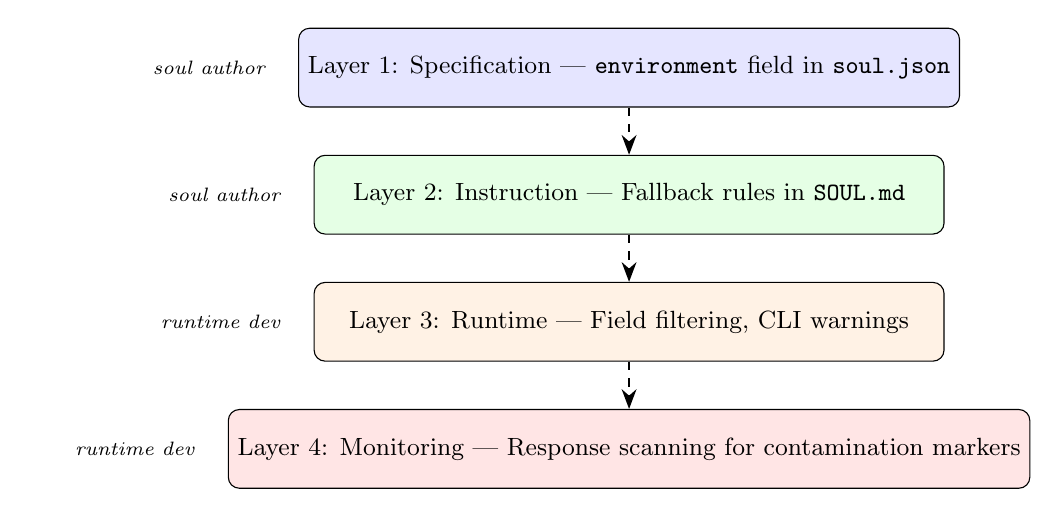
\begin{tikzpicture}[
    node distance=0.6cm,
    layer/.style={rectangle, draw, rounded corners, minimum width=8cm, minimum height=1.0cm, align=center, font=\small},
    arrow/.style={-{Stealth[length=2.5mm]}, thick, dashed},
]
\node[layer, fill=blue!10] (L1) {Layer 1: Specification --- \texttt{environment} field in \texttt{soul.json}};
\node[layer, fill=green!10, below=of L1] (L2) {Layer 2: Instruction --- Fallback rules in \texttt{SOUL.md}};
\node[layer, fill=orange!10, below=of L2] (L3) {Layer 3: Runtime --- Field filtering, CLI warnings};
\node[layer, fill=red!10, below=of L3] (L4) {Layer 4: Monitoring --- Response scanning for contamination markers};

\node[left=0.3cm of L1, font=\scriptsize\itshape, text width=2cm, align=right] {soul author};
\node[left=0.3cm of L2, font=\scriptsize\itshape, text width=2cm, align=right] {soul author};
\node[left=0.3cm of L3, font=\scriptsize\itshape, text width=2cm, align=right] {runtime dev};
\node[left=0.3cm of L4, font=\scriptsize\itshape, text width=2cm, align=right] {runtime dev};

\draw[arrow] (L1) -- (L2);
\draw[arrow] (L2) -- (L3);
\draw[arrow] (L3) -- (L4);
\end{tikzpicture}
\caption{Defense-in-depth strategy for cross-modal persona contamination. Each layer independently reduces contamination risk; combined, they provide robust protection.}
\label{fig:defense}
\end{figure}

\textbf{Layer 1: Specification-level.}
The \texttt{environment} field in \texttt{soul.json} declares the intended deployment modality.
This is the most fundamental mitigation: it provides machine-readable metadata that downstream systems can act upon.

\textbf{Layer 2: Instruction-level.}
Natural-language fallback instructions in \texttt{SOUL.md} direct the LLM to ignore physical fields when operating in a text-only context.
This layer is critical for runtimes that ingest the full specification as text without structured parsing.

\textbf{Layer 3: Runtime-level.}
Modality-aware runtimes could filter modality-irrelevant fields before LLM ingestion, emit operator warnings on modality mismatch, and validate soul compatibility at load time (e.g., a hypothetical \texttt{soul validate --runtime=text} CLI command).

\textbf{Layer 4: Monitoring.}
Post-generation response scanning can detect contamination markers (physical attribute references, hardware identifiers, sensor/actuator keywords) and flag or suppress contaminated responses.

The recommended pattern combines all four layers:
\begin{enumerate}
    \item Soul author sets \texttt{environment} field.
    \item Soul author includes fallback instructions in \texttt{SOUL.md}.
    \item Runtime filters fields based on \texttt{environment} and current modality.
    \item Runtime monitors responses for residual contamination.
\end{enumerate}


% ============================================================
\section{Discussion}
\label{sec:discussion}
% ============================================================

\subsection{Implications for Persona Specification Standards}

Our findings suggest that \emph{all} persona specification formats should include modality metadata.
The \texttt{AGENTS.md} format studied by Lulla et al.~\cite{jai2025agents} achieves impressive efficiency gains, but implicitly assumes a text-based coding environment.
As the same configuration patterns extend to embodied agents, modality awareness becomes necessary.
\textsc{Soul Spec} can be viewed as a superset of \texttt{AGENTS.md} with explicit modality support: the \texttt{environment} field and progressive disclosure mechanism address a concern absent from current agent configuration standards.

\subsection{Format Matters: JSON vs.\ Natural Language}

Our observation that contamination severity varies across runtimes (S2: CR\,=\,0.60 on ChatGPT vs.\ 0.90 on Claude.ai) has implications for specification design.
Structured formats may provide a degree of implicit contamination resistance: LLMs trained on JSON schemas may be more likely to treat unknown fields as data rather than behavioral instructions.
This suggests a design principle: \emph{modality-specific attributes should be specified in structured formats, not prose}.

\subsection{The Scaling Problem}

Cross-modal contamination scales with specification complexity.
A simple soul with one physical field (e.g., \texttt{maxSpeed}) produces minimal contamination.
A rich embodied soul with dozens of sensors, actuators, and safety rules creates a substantial ``contamination surface.''
As soul specifications grow to support increasingly sophisticated embodied agents---dexterous manipulators, autonomous vehicles, surgical robots---the contamination risk increases proportionally without systematic mitigation.

\subsection{Broader Context}

The convergence of text-based AI assistants and embodied robots around shared LLM backends makes cross-modal deployment increasingly likely.
A care companion robot and its text-based fallback interface may share the same soul specification.
A warehouse automation system and its remote monitoring chatbot may use the same agent configuration.
In each case, cross-modal persona contamination represents a concrete usability failure---and in safety-critical domains, potentially a safety hazard (e.g., a text interface claiming it has stopped moving when no physical robot is involved).


% ============================================================
\section{Limitations and Future Work}
\label{sec:limitations}
% ============================================================

\textbf{Pilot scale.}
Our findings are based on a structured pilot ($n=40$ instances) scored by the first author without blinding.
We have not conducted the proposed large-scale experiment (Section~\ref{sec:experiment}).
Contamination rates should be treated as directional indicators pending larger-sample replication with multiple independent raters.

\textbf{Limited runtimes.}
We tested only two runtimes (ChatGPT and Claude.ai).
Results may differ substantially across other LLM backends (Claude, Gemini, open-weight models) and runtime architectures.

\textbf{No user study.}
We assessed contamination objectively (presence of physical attribute references) but did not measure user perception or downstream effects on task performance.

\textbf{Evolving LLM capabilities.}
LLM behavior changes with model updates.
Contamination patterns observed with current models may not persist in future versions, particularly as models become better at schema-aware context processing.

\textbf{Future work.}
We plan to: (1)~execute the proposed experimental design with $N \geq 100$ prompts across 5+ runtimes; (2)~conduct a user study measuring perceived persona coherence under cross-modal conditions; (3)~develop automated contamination detection tools integrated into \textsc{OpenClaw}'s soul validation pipeline; and (4)~extend the taxonomy as new contamination patterns emerge with more complex embodied specifications.


% ============================================================
\section{Conclusion}
\label{sec:conclusion}
% ============================================================

We have identified cross-modal persona contamination as a previously uncharacterized failure mode that arises when embodied AI agent configurations are loaded into text-only runtimes.
Our taxonomy of five contamination types---attribute leakage, behavioral mismatch, safety confusion, identity pollution, and capability hallucination---provides a framework for understanding and measuring this phenomenon.

Pilot experimental results across ChatGPT and Claude.ai confirm that contamination occurs in practice (S2 CR\,=\,0.60--0.90 without mitigation).
Instruction-level fallback mitigations reduce contamination significantly (S3/S4 CR\,$\leq$\,0.40), though attribute leakage persists.
These findings motivate the defense-in-depth strategy proposed in Soul Spec~v0.5, which adds specification-level (the \texttt{environment} field), runtime-level (progressive disclosure), and monitoring-level protections beyond the instruction-level mitigations tested here.

As AI persona specifications evolve to support both text and embodied agents, modality must be treated as a first-class citizen in specification design.
The \texttt{environment} field pattern is a minimal, backward-compatible mechanism that enables this.
We invite the research community and specification authors to adopt modality-aware persona design and to validate our pilot findings through rigorous empirical study.

\section*{Acknowledgments}
This paper was drafted with assistance from Claude (Anthropic). All claims, experimental observations, references, and conclusions were manually verified by the author.

\bibliographystyle{ACM-Reference-Format}
\bibliography{cross-modal-refs}

\end{document}
